\documentclass[11pt,a4paper]{article}
\title{Behaviour Analysis of Elderly using topic models}
\author{Kristin Rieping}
\usepackage[latin1]{inputenc}
\usepackage{amsmath}
\usepackage{amsfonts}
\usepackage{amssymb}
\usepackage{graphicx}

\usepackage{cite}
\usepackage{natbib}
\begin{document}

\maketitle
%----------------------------------INTRODUCTION--------------------------------------------
\section{Introduction}
The world population increases unceasingly and thereby the percentage of elderly also increases. The manpower to take care of elderly is diminishing. So it becomes more and more important to give elderly the opportunity to live on there own and be more independent of health care.
New techniques give the possibility to monitor elderly from the distance or even automatically. Some of these techniques use cameras that are placed in the homes of elderly. But these methods are privacy-sensitive and often not adopted by the elderlies. []
Other methods use motion sensors that are placed at different locations in the homes of elderly. 
Reading and interpreting this sensor data is often difficult and that is why often activity recognition is done to make the data more readable. But different approaches show that this is also a though challenge. [ ]
Machine Learning techniques often require a lot of annotated data, but the task of labeling a data set is time consuming and and can also influence the output of the data while doing so.\\
Therefore we focus in this thesis on finding features in an unsupervised manner. These features should be meaningful and easy to interpret. We do not focus so much on activity recognition but look more widely on the daily behavior of a person. As an inspiration we use the analysis of human routines described in \cite{farrahi2008daily} .  With an EM-algorithm for Latent Dirichlet Allocation (LDA) we try to distinguish topics in binary sensor data. The topics should describe different behaviors in the daily routines of a person. The LDA algorithm described in  \cite{blei2003latent}  is adjusted to fit the given data.

The data that we use is received in the same way as described in \cite{van2010activity}, except that our data is not annotated.
%--------------------------------METHOD:LDA-----------------------------------------------
\section{Topic model for daily behavior of people in home environments}
%In this section we give a global overview how we analyze the daily behavior in peoples life. First we give an introduction of the data that is used. Then we introduce the topic model that captures the behaviors. We go in more detail about the topic model 'Latent Dirichlet Allocation' and how we use it. We also describe the problems that this approach has and how they can be solved.




\subsection{Topic Models for behavior Analysis}
The binary data received from motion sensors in homes are complex and it appears to be difficult to read and also interpret for  professionals in the health care. who want to analyze the data. It is for example not interesting to know that when exactly and for how long the microwave is used. It would make more sense to know if some ate his breakfast or not.
Therefore it is important to simplify the data in such a way, that it is easy to interpret and to read.\\
With a topic model, which is often used in document classifying, this might be possible. With such a model a day in a persons life can be described with a combination of topics. Possible topics might be  'Getting up early'. 'Eating breakfast' or 'Toileting often'. Such information could give valuable information to the health professionals that need to take care for an elderly. If for example the behavior changes, this might be a sign of an illness and the health professional can act to it adequate.

\subsection{Data description}
The sensors that are placed in the homes of elderly are placed at different locations, for example at doors, cupboards, microwave, toilet flush or several other places that a frequently used. Several sensors are grouped together and form a field. In the following descriptions we use five fields, which are $\{$'kitchen','living room','bathroom','bedroom','hallway'$\}$. The sensors that define a field can differ between different homes and are specified manually.
From the sensors we receive the time when it is triggered and in which value it changes to. Possible values are $\{$0,1$\}$. In figure~\ref{fig:PlaineSensorData} an example of the sensor datafor one day is shown.\\

\begin{figure}[h!]
  \centering
    	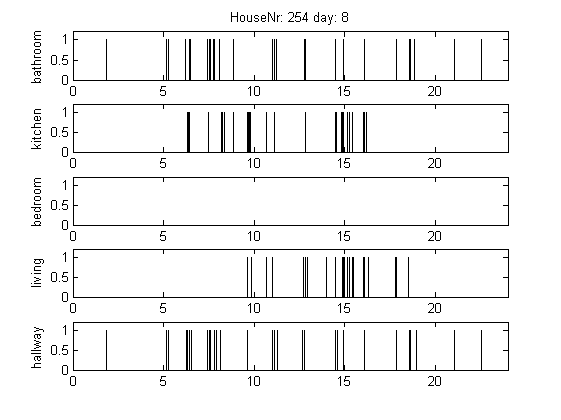
\includegraphics[width=0.7\textwidth]{Pictures/plainDataExample.png}
    \caption{Sensor Data for one day with five fields}
    \label{fig:PlaineSensorData}
\end{figure}


In a first approach we discretize the data into time-slices of half an hour. In each time-slice we count the amount of sensor activations in all the fields. We do not take the length of sensor activities into account. That means that a time-slice can be represented as a vector $w_n$ of length five, for every field a value $v_i>=0$ element N(hele getallen). We add an additional dimension to the vector to capture the the time in which the observation is taken. The values lay between 1 and 48, for every time-slice a value. This is necessary to model the time dependency from the data, which is not automatically captured in the topic model that we are going to use. The dimension of an observation will become $d=6$. We say that a day starts at 3 a.m. so that we reduce the chance to cut between activities. It still can occur that a person goes to bed late or that he needs to visit the toilet, but we will ignore this fact for now.



\subsection{Latent Dirichlet Allocation for behavior Analysis}
The generative model 'Latent Dirichlet Allocation' [Blei] is a way to describe a topic model. In this model it is assumed that a Corpus can be generated from a distribution of topics, where every topic is a distribution of words.
In our case the Corpus is a set of days and every day is representing a document. The observations $w_n$ represents the words in the model. The dictionary $V$ will be the set of all seen observations. The generative process that could create the data will look like this:

For every day that will be generated:\\
1. Set the amount of time-slices in every document to size N (for every document the same).
2. Choose a topic distribution $\theta \sim Dir(\alpha)$ for the day.\\
3. For each of the N time-slices $w_n$:\\
(a) Choose a topic $z_n \sim Multinomial(\theta)$.\\
(b) Choose a set of obeservations $w_n$ from the set of all observations $V$ from $p(w_n |z_n;\beta)$, a multinomial probability conditioned on the topic $z_n$. Where $\beta$ is the distribution over observations given a topic.\\

With the assumption that the data that we got from the sensor system has the same structure than the data created with the generative process we can try to find the model parameters for LDA as described in [Blei].

\subsection{K-means}
In our data the size of the dictionary, which contains all unique observations in the whole corpus is relative large with respect to the size of the data that we have. There are a lot of different observations that are similar to each other, but differ only in one value of the 6 dimensions. The LDA model does not group similar observations together and therefore LDA can not find good model parameters.
A simple way is to cluster all observations together and then again use the EM-algorithm to estimate the parameters of the  LDA model. We use the k-means algorithm to find the best clusters. With this approach we can reduce the dictionary size and may find better results.


\subsection{Extension of LDA model}
Preprocessing the data with k-means may may not capture the topic distributions probably. So we want to avoid the preprocessing the data with k-means and add the the clustering part directly in the model. This is done in the following way:
Instead of storing the probability for a observation given a topic, which is done in the matrix $\beta$, we assume that every dimension of the observations is normal distributed given a topic. So we store the mean and variance for every dimension given a topic in two matrices of size $d \times k$ where $d$ is the dimension of the observations and $k$ the amount of clusters. For now we assume that the dimensions of the observations are uncorrelated. The EM-algorithm is adjusted to calculate the $\beta$- matrix properly.

Note:
I think that the model does not capture the mixtures of words that specify a topic well. A topic that mainly be specified by two words in the main model, can not be well defined with one gaussian (in every dimension). A better way would be a mixture of gaussians for every topic, but this is I think kind of hard to model with so little data.\\
Further, I did not find all references I want to add.


\bibliography{research}

\bibliographystyle{plain}


\end{document}
